\documentclass[10pt]{beamer}
\usepackage{listings}
\usetheme{uha}
\usepackage{hyperref}
\usepackage{indentfirst}
\usepackage{booktabs}
\usepackage{multirow}
\usepackage{xeCJK}
\usepackage[french,english]{babel}
\usepackage[T1]{fontenc}
\usepackage[utf8]{inputenc}
\usepackage{amsmath}
\usepackage{amsfonts}
\usepackage{amssymb}
\usepackage{tikz}
\usepackage{enumerate} %枚举宏包
\usepackage{geometry}
\usepackage{xcolor}
\punctstyle{kaiming}

\definecolor{mygray}{rgb}{0.3,0.3,0.3}
\definecolor{codegreen}{rgb}{0.8,0.8,0.8}
\title{Body Area Network}
\subtitle{Demo Test Report}
\date{\today}
\author{ ZZDC SW }
\institute{Foxconn ZZDC}
\setmainfont{Times_New_Roman.ttf}
\lstset{
	numbers=left,
	numberstyle=\tiny,
	basicstyle=\scriptsize,
	backgroundcolor= \color{gray},
	keywordstyle=\color{blue!70},
	breaklines=true,
	breakautoindent=true,
	breakindent=4em,
	commentstyle=\color{codegreen},
	frame=shadowbox,
	escapeinside=``,
	tabsize=4,
	framextopmargin=1pt,framexbottommargin=1pt,abovecaptionskip=-1pt,belowcaptionskip=1pt,
  xleftmargin=3em,xrightmargin=3em,
	language=C
}


\begin{document}




% Title page 标题页
\begin{frame}[plain, noframenumbering]
	\titlepage
\end{frame}


\section{Introduce}

%------------------------------------------------
\begin{frame}[fragile]{ RS485 feature}

\begin{itemize}
\item  485 is  Fully balanced
\item 485 handles multiple drivers and receivers
\item Better common-mode noise rejection (-7 to +12Volts)
\item Sensitivity of 200mV in receivers
\item Drivers give up to 5 volts balanced output
\item Can stand contention, driver shuts down by itself
\item High input resistance (12K ohms)
\item Hysteresis of 50 mv to overcome diff. noise
\end{itemize}

\begin{figure}[htbp]
\begin{center}
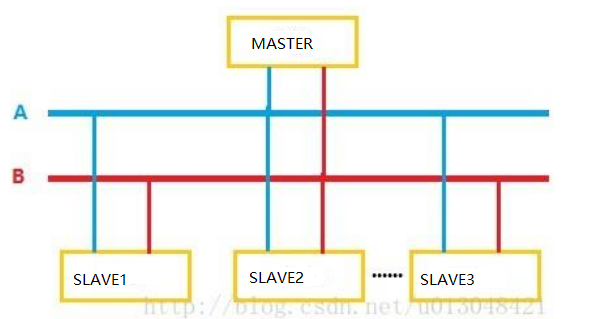
\includegraphics[width=5cm]{img/485net}
\caption{485NET }
\label{Overview}
\end{center}
\vspace{-0.5em}
\end{figure}

\end{frame}


%------------------------------------------------
\begin{frame}[fragile]{The Principle of The BAN's Clock Synchronization}

\begin{itemize}
  \item In order to synchronize the device clock, it is necessary to add a clock line between Master and Slave, where Master generates synchronous clock square wave.
\end{itemize}

\begin{figure}[htbp]
\begin{center}
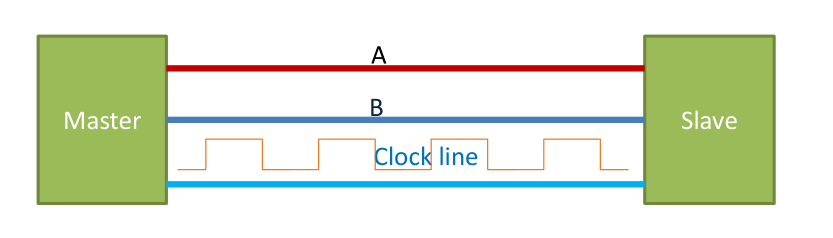
\includegraphics[width=6cm]{img/syncchart}
\caption{synchronous}
\label{Overview}
\end{center}
\vspace{-0.5em}
\end{figure}
\end{frame}


%------------------------------------------------
\begin{frame}[fragile]{Our Design}
We designed it like this:
\begin{figure}[htbp]
\begin{center}
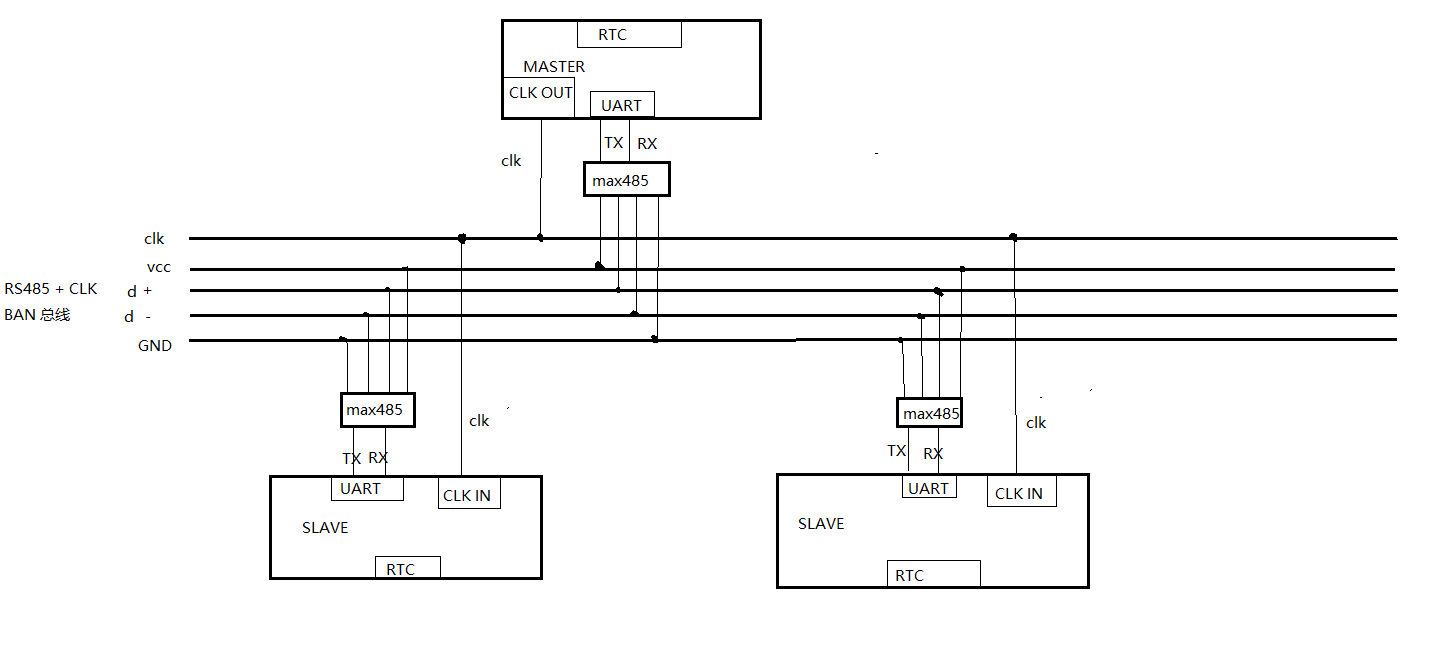
\includegraphics[width=10cm]{img/overview}
\caption{BAN }
\label{Overview}
\end{center}
\vspace{-0.5em}
\end{figure}
\end{frame}





%------------------------------------------------
\begin{frame}[fragile]{BUS}

\begin{enumerate}
\item Adding a clock line from RS485 to form the basic hardware circuit of BAN bus.
\item The clock  line is used to generate Millisecond-level pulses for clock synchronization.Later aliases:SYNC\_CLK
\item D +, D - is  differential  signal  .

\end{enumerate}

we assumed that the device mounted on the bus has one Master and two Slaves.


\end{frame}

%------------------------------------------------
\begin{frame}[fragile]{Local Clock Counter \& SYNC\_CLK}

\begin{itemize}
\item  Local Clock Counter , Each device has a local clock counter. The timing granularity is 100us.

\item  SYNC\_CLK,The device on BAN bus uses clock line to complete clock synchronization. Master's timer generates synchronization pulse, Slave'scaptures synchronized  pulse to complete synchronization.
\end{itemize}


\end{frame}





%------------------------------------------------
\begin{frame}[fragile]{Synchronization process}

\begin{itemize}
\item a. master and slave power on and initialize peripherals.
\item b. master starts sending square wave signals,at The first rising edge of
square wave signal:
  \begin{enumerate}
    \item  The master starts Master's Local Clock Counter(MLCC).
    \item Slave captures this rising edge at the same time.Then start Slave's Local Clock Counter(SLCC).
    \item The delay of the rising edge of the clock line transmission can be neglected, So we think that MLCC and SLCC start counting at the same time.
  \end{enumerate}
 \item c. Slave calibrates SLCC at each subsequent SYNC\_CLK rising edge.

\end{itemize}



\begin{figure}[htbp]
\begin{center}
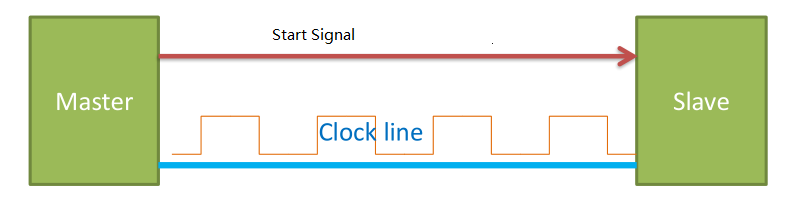
\includegraphics[width=6cm]{img/abstim}
\caption{BAN }
\label{Overview}
\end{center}
\vspace{-0.5em}
\end{figure}
\end{frame}





%------------------------------------------------
\begin{frame}[fragile]{Clock Difference Calibration}

SYNC\_CLK is produced by Master with fixed period and precise time.Let's take a period of 16 milliseconds for example.

MLLC and SLLC start counter at the sametime(first SYNC\_CLK rising edge). Their timing granularity is small, 100 microseconds.

So when the system runs, there are two counts on each device, the Local Clock Count(Every 100 microseconds plus 1) and the SYNC\_CLK Count(Every 16 milliseconds plus 160).Slave calibrates SLCC at each subsequent SYNC\_CLK rising edge by Make those two counts the same.



\end{frame}




%------------------------------------------------
\begin{frame}[fragile]{Clock Difference Calibration}

  \begin{figure}[htbp]
  \begin{center}
  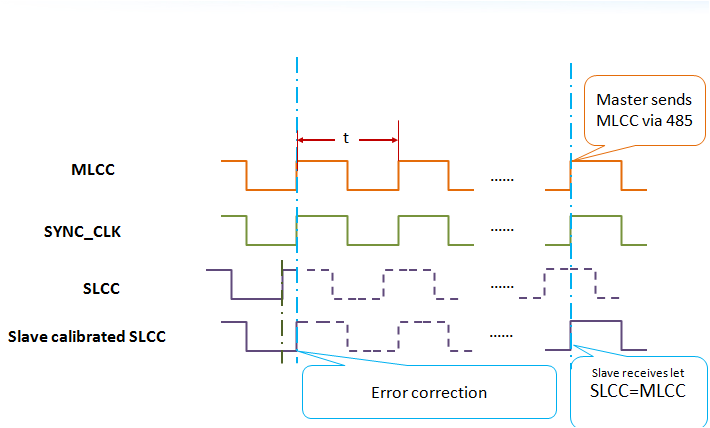
\includegraphics[width=10cm]{img/flow}
  \caption{BAN }
  \label{Overview}
  \end{center}
  \vspace{-0.5em}
  \end{figure}

\end{frame}






%------------------------------------------------
\begin{frame}[fragile]{Demo implementation}

The following is the demo wiring and structure:
\begin{figure}[htbp]
\begin{center}
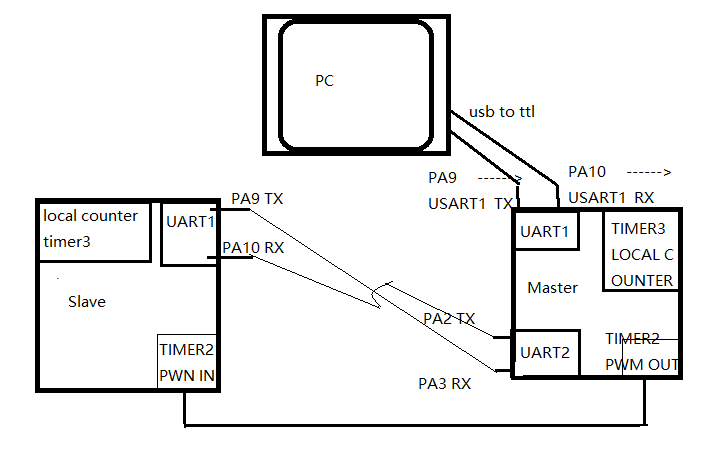
\includegraphics[width=10cm]{img/demo0}
\caption{demo}
\label{Overview}
\end{center}
\vspace{-0.5em}
\end{figure}

\end{frame}

\section{workflow}

%------------------------------------------------
\begin{frame}[fragile]{Demo workflow}

\begin{enumerate}
\item Master and Slave Power on。 Peripheral Driver Initialization
\item The Master sends a synchronization command, when ensuring that the slave is online:
  \begin{itemize}
    \item a.start timer2 to Generating Pulse Square Wave for synchronous。
    \item b. start  timer3 for  MLCC(Master Local Clock Counter).
  \end{itemize}
\item When Slave receives a synchronization command from Master, and Slave captures the first rising edge of SYNC\_CLK:
  \begin{itemize}
    \item a.  start  timer3 for  SLCC(Slave Local Clock Counter).
    \item b. Continue to capture the rising edge.

  \end{itemize}


\end{enumerate}


\end{frame}


%------------------------------------------------
\begin{frame}[fragile]{Demo Workflow: Synchronize details}

local\_tm\_t is the type of time described in Master and Slave code:

\begin{lstlisting}
typedef struct local_time_struct{
 unsigned char sec:7;   //second
 unsigned char min:7;   //min
 unsigned char hour:5;  //hour
 unsigned int  day;     //day
 unsigned int  jiffies; //LCC
 unsigned int  jiffies_pwm;   //SYNC_CLK counter
} local_tm_t;
\end{lstlisting}



\end{frame}



%------------------------------------------------
\begin{frame}[fragile]{Slave Rising Edge Capture Interrupt}

tick\_sync is called every 8ms to synchronize the local timestamp:

\begin{lstlisting}
/* every 8ms 80*100us  */
void tick_sync(void)
{
  if( dev.local_tm.jiffies_pwm + 80 < 10000  ){
  dev.local_tm.jiffies_pwm = dev.local_tm.jiffies_pwm  + 80;
  }
  if( dev.local_tm.jiffies_pwm + 80 >= 10000  ){
    dev.evt.sec_need_update=1;
    dev.local_tm.jiffies_pwm = 80 - (10000 - dev.local_tm.jiffies_pwm);
  }
  dev.local_tm.jiffies = dev.local_tm.jiffies_pwm;		//synchronous
}
\end{lstlisting}

\end{frame}



%------------------------------------------------
\begin{frame}[fragile]{Synchronize details:test point}

Enter this code  every 100us:
\begin{lstlisting}
/*
 enter this code  every 100us。
*/
void Tick(void)
{
  dev.local_tm.jiffies ++;
  if( dev.local_tm.jiffies % 80 == 0){
   //GPIO A5 for compare.
   HAL_GPIO_WritePin(GPIOA,GPIO_PIN_5,1-HAL_GPIO_ReadPin(GPIOA,GPIO_PIN_5));
 }
  /* one second passed */
  if(dev.local_tm.jiffies >= 10000 ){
   dev.local_tm.jiffies  = 0;
 }
}
\end{lstlisting}
Here the slave GPIOA5 has square wave output relative to the clock synchronization line. It's a test point.
\end{frame}

\section{TEST Data}




%------------------------------------------------
\begin{frame}[fragile]{Waveform: Unsynchronized}

Let:
\begin{itemize}
  \item The local clock inverts the GPIOA5 level state every 8ms. This test channel is marked CH\_LOCAL.

  \item The synchronous line generates a synchronous square wave with a half period of 8ms from the Master. This test channel is marked CH\_SYNC.

  \item In the interrupt processing function of the slave to capture the rising edge of the synchronization line, the clock is not synchronized, that is to say, the following code is commented out:

  \begin{lstlisting}
//dev.local_tm.jiffies = dev.local_tm.jiffies_pwm;		//synchronize code
  \end{lstlisting}

\end{itemize}

The following screenshots show the unsynchronized screenshots:


\end{frame}


%------------------------------------------------
\begin{frame}[fragile]{Waveform: Unsynchronized}

Unsynchronized waveform 1\label{nosyncwave1}:

  \begin{figure}[htbp]
  \begin{center}
  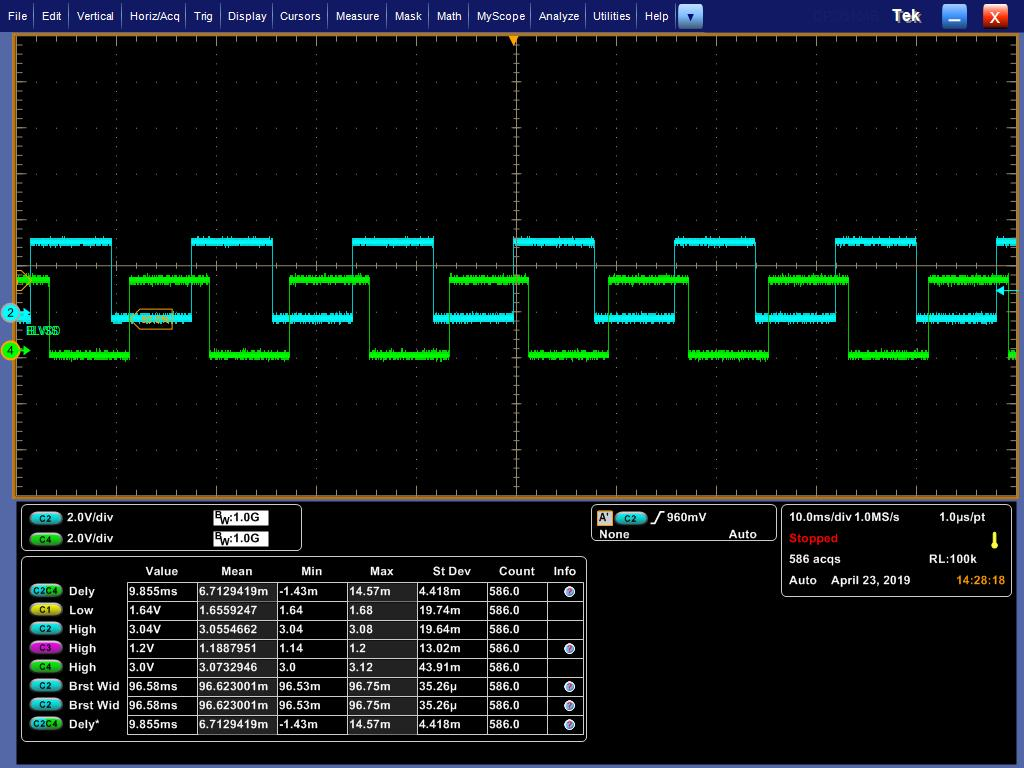
\includegraphics[width=10cm]{img/nosync1}
  \caption{nosync1}
  \label{report}
  \end{center}
  \vspace{-0.5em}
  \end{figure}


\end{frame}



%------------------------------------------------
\begin{frame}[fragile]{Waveform: Unsynchronized}

Unsynchronized waveform 2:

  \begin{figure}[htbp]
  \begin{center}
  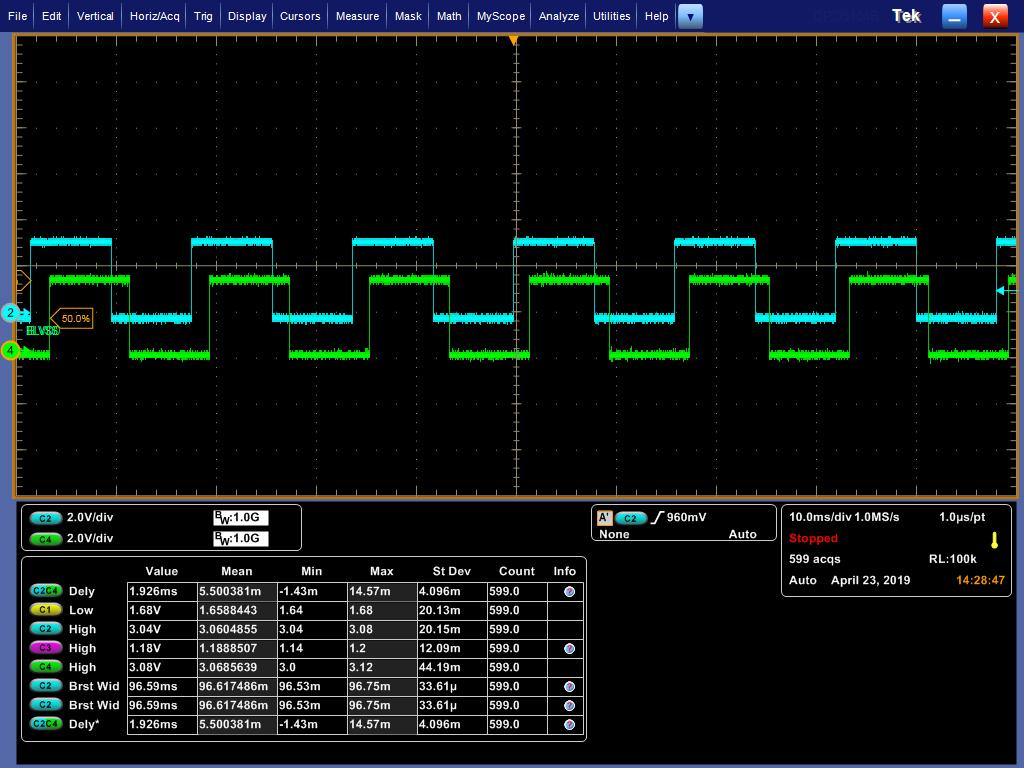
\includegraphics[width=10cm]{img/nosync2}
  \caption{nosync2}
  \label{report}
  \end{center}
  \vspace{-0.5em}
  \end{figure}


\end{frame}


%------------------------------------------------
\begin{frame}[fragile]{Waveform: Unsynchronized}

Unsynchronized waveform 3:

  \begin{figure}[htbp]
  \begin{center}
  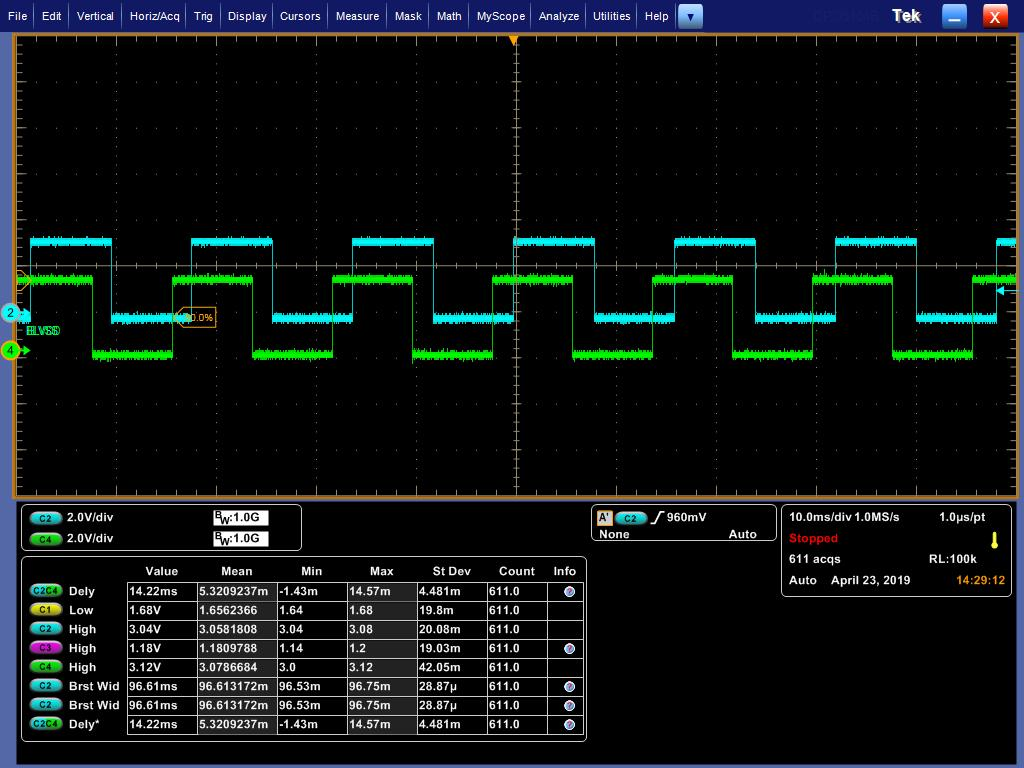
\includegraphics[width=10cm]{img/nosync3}
  \caption{nosync3}
  \label{report}
  \end{center}
  \vspace{-0.5em}
  \end{figure}


\end{frame}


%------------------------------------------------
\begin{frame}[fragile]{Waveform: Unsynchronized}

Unsynchronized waveform 4:

  \begin{figure}[htbp]
  \begin{center}
  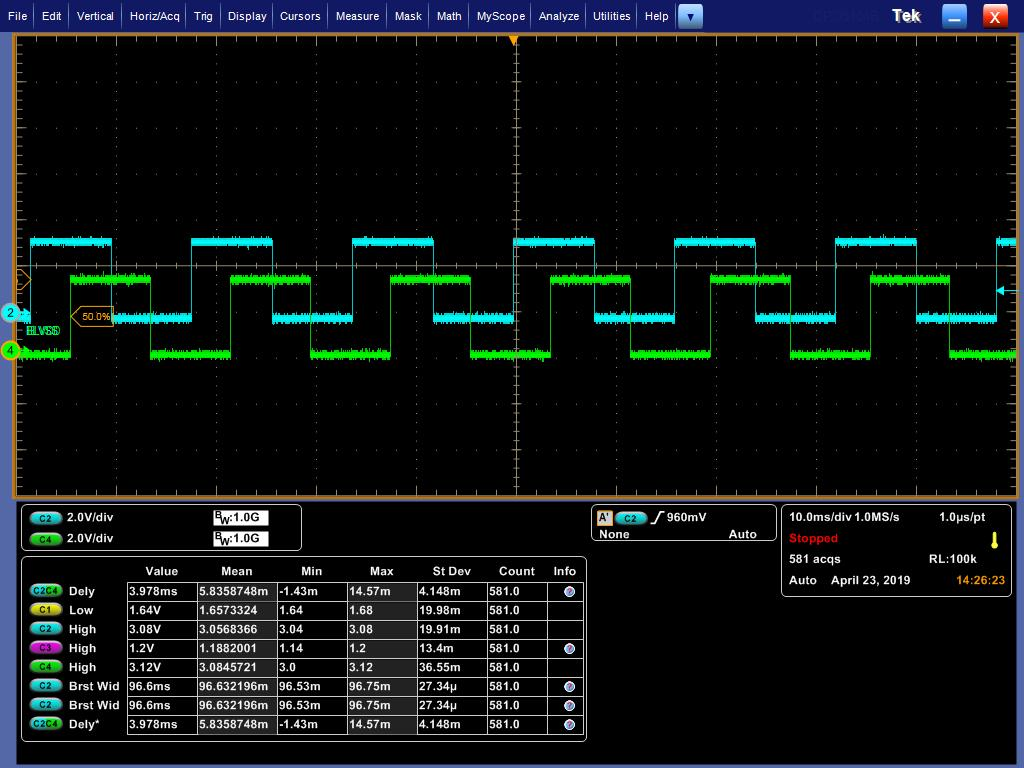
\includegraphics[width=10cm]{img/nosync4}
  \caption{nosync4}
  \label{report}
  \end{center}
  \vspace{-0.5em}
  \end{figure}


\end{frame}


%------------------------------------------------
\begin{frame}[fragile]{Some explanations of unsynchronized waveforms}


Return this document to unsynchronized waveform 1 ( \ref {nosyncwave1}) and turn the page with the right key of the keyboard direction key (from unsynchronized waveform 1 to unsynchronized waveform 4). At this time, the animation effect on the screen can restore the appearance of the oscilloscope at that time.

Because the local clock is not synchronized, each difference accumulates, resulting in such a dynamic effect.


\end{frame}



%------------------------------------------------
\begin{frame}[fragile]{Waveform: Synchronization }
Let:
\begin{itemize}
  \item The local clock inverts the GPIOA5 level state every 8ms. This test channel is marked CH\_LOCAL.

  \item The synchronous line generates a synchronous square wave with a half period of 8ms from the Master. This test channel is marked CH\_SYNC.
  \item In the interrupt processing function of the slave capturing the rising edge of the synchronization line, the clock is synchronized, that is to say, the following code is active:

  \begin{lstlisting}
dev.local_tm.jiffies = dev.local_tm.jiffies_pwm;		//synchronize code
  \end{lstlisting}

\end{itemize}

The following screenshots show the screenshots in the case of synchronization.

\end{frame}


%------------------------------------------------
\begin{frame}[fragile]{Waveform: Synchronization}

synchronized waveform :

  \begin{figure}[htbp]
  \begin{center}
  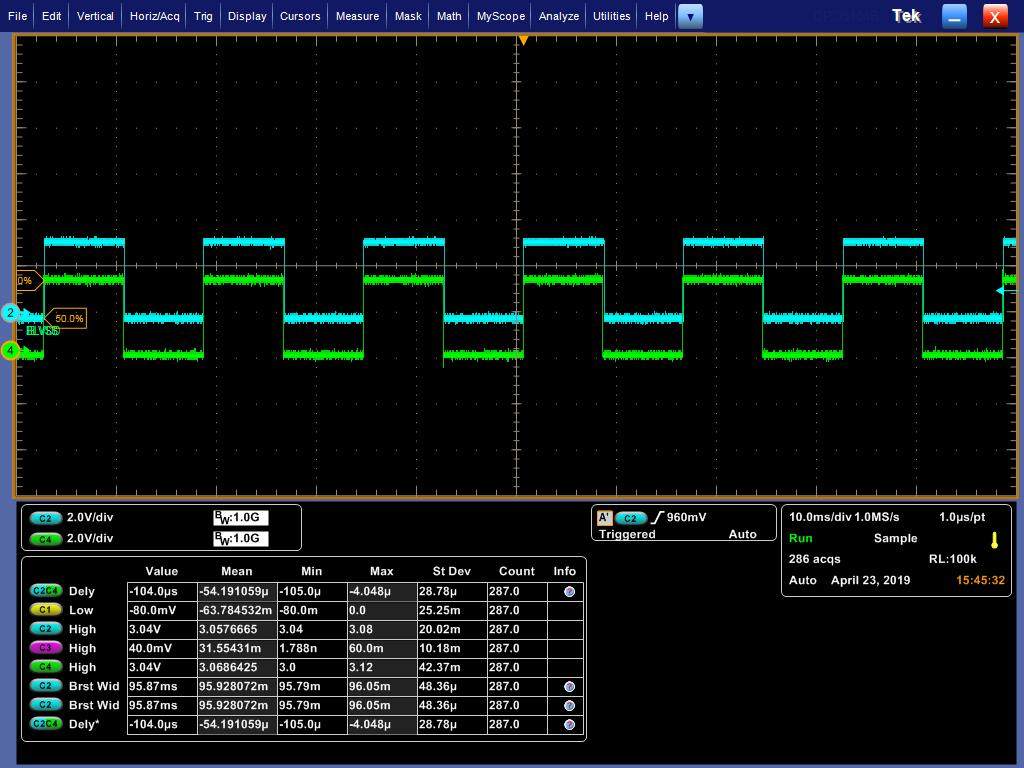
\includegraphics[width=10cm]{img/sync}
  \caption{report jiffies}
  \label{report}
  \end{center}
  \vspace{-0.5em}
  \end{figure}


\end{frame}

%------------------------------------------------
\begin{frame}[fragile]{Waveform: Synchronization}

Since the rising edge of each synchronization line is captured by slave computer, synchronization interrupt will be triggered. In interrupt processing, the local clock error of each cycle will be eliminated.


So the synchronized waveform looks fixed  and the phase is relatively consistent. But:

If we amplify the size of the oscilloscope, we will find that there are difference. The following are some synchronization delay. The size of the oscilloscope is already 50us. We are concerned about the synchronization time.


\end{frame}



%------------------------------------------------
\begin{frame}[fragile]{Waveform: Synchronization}

Synchronization delay:

  \begin{figure}[htbp]
  \begin{center}
  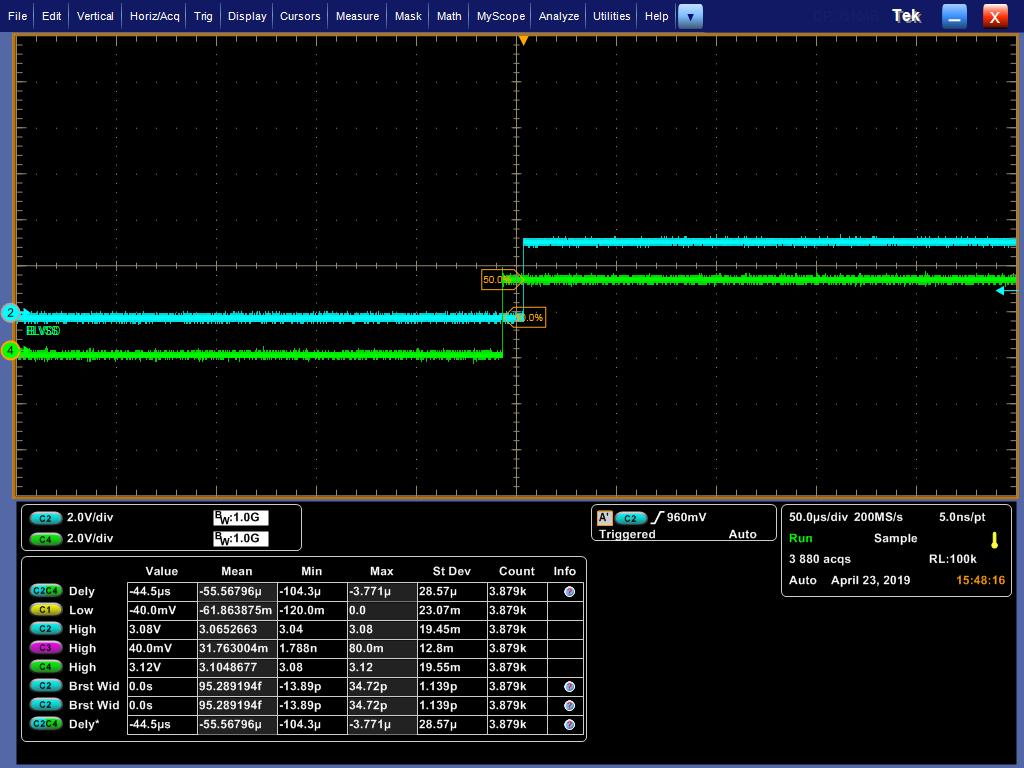
\includegraphics[width=10cm]{img/mis1}
  \caption{Synchronization delay1}
  \label{report}
  \end{center}
  \vspace{-0.5em}
  \end{figure}


\end{frame}


%------------------------------------------------
\begin{frame}[fragile]{Synchronization delay}

Synchronization delay:

  \begin{figure}[htbp]
  \begin{center}
  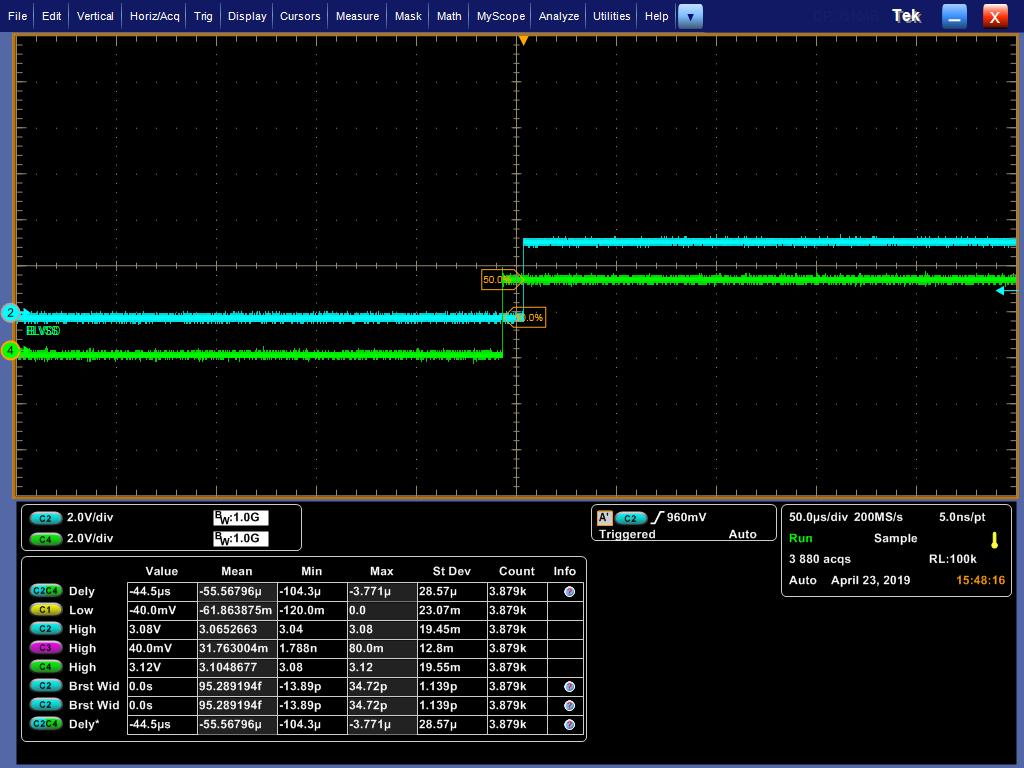
\includegraphics[width=10cm]{img/mis1}
  \caption{Synchronization delay1}
  \label{report}
  \end{center}
  \vspace{-0.5em}
  \end{figure}


\end{frame}
%------------------------------------------------
\begin{frame}[fragile]{Synchronization delay}

Synchronization delay:

  \begin{figure}[htbp]
  \begin{center}
  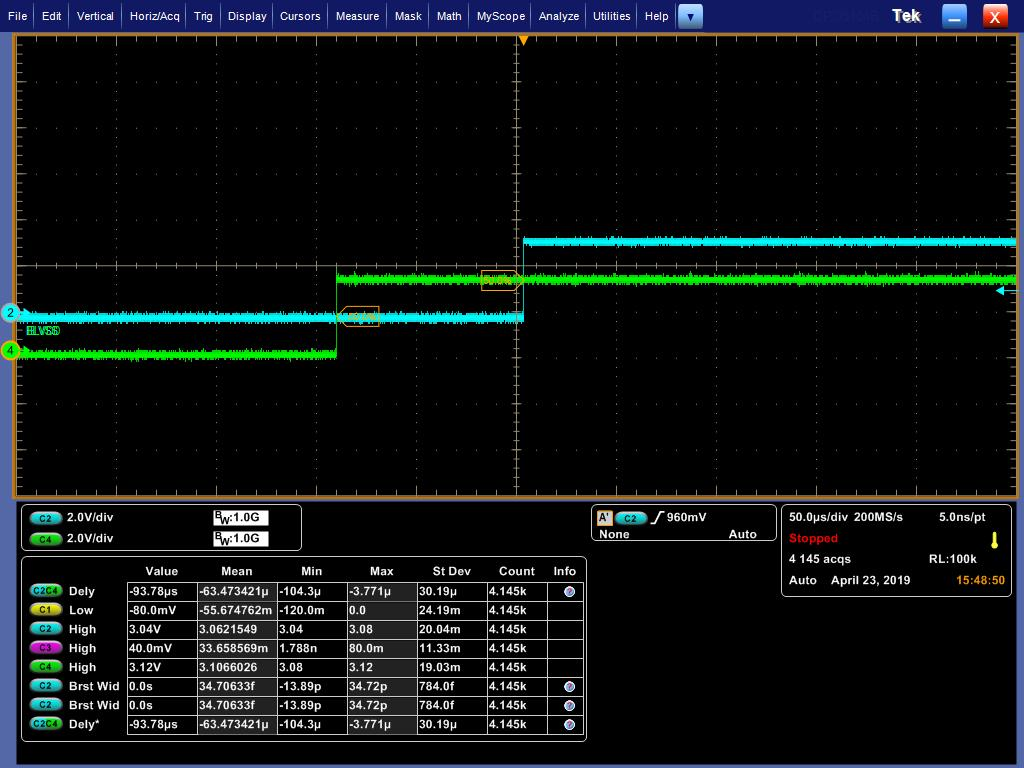
\includegraphics[width=10cm]{img/mis2}
  \caption{Synchronization delay2}
  \label{report}
  \end{center}
  \vspace{-0.5em}
  \end{figure}


\end{frame}

%------------------------------------------------
\begin{frame}[fragile]{Synchronization delay}

Synchronization delay:

  \begin{figure}[htbp]
  \begin{center}
  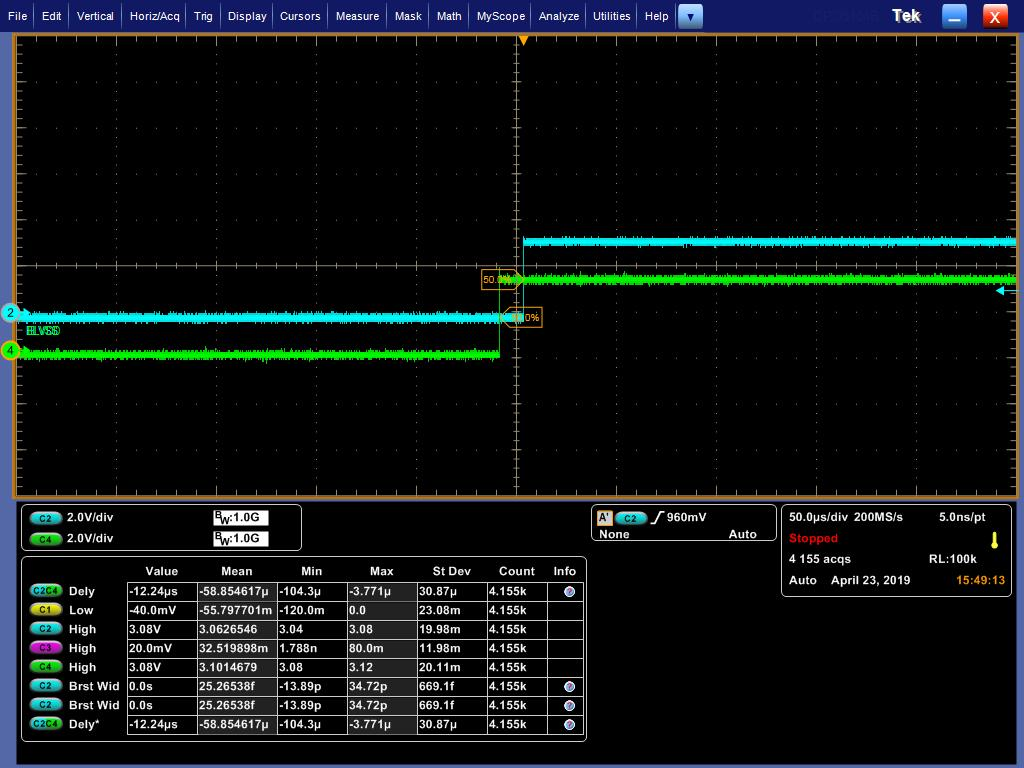
\includegraphics[width=10cm]{img/mis3}
  \caption{Synchronization delay3}
  \label{report}
  \end{center}
  \vspace{-0.5em}
  \end{figure}

\end{frame}


%------------------------------------------------
\begin{frame}[fragile]{Synchronization delay}

  \begin{figure}[htbp]
  \begin{center}
  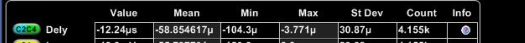
\includegraphics[width=7cm]{img/delay}
  \caption{delay}
  \label{report}
  \end{center}
  \vspace{-0.5em}
  \end{figure}


As can be seen from the figure above, the maximum phase difference between CH\_LOCAL and CH\_SYNC is -3.771 -(-104.3) = 100.529us  when sampling 4.155k times.

\end{frame}


%------------------------------------------------
\begin{frame}[fragile]{summary}

Data transmission through serial ports can cause some delays (although there is no blocking at the time of sending, receiving in the interrupt, reading registers directly). The baudrate we used in this example is 115200*2 bps.



Software-only CRC verification will inevitably lead to a certain delay. If it is necessary to verify, the driver of CRC hardware peripherals should be realized in this project.

The error of demo synchronization has been tested many times, among which there are transformed master-slave roles, and the maximum error is less than 500 us. The most common is within 300us.

The test code logic is not complex, real-time processing is in the interrupt context, and STM32F4 uses Cortex M4's Nested Vectored Interrupt Controller (NVIC) real-time is very high, there should be little optimization space.

\end{frame}




\end{document}
